% !TEX root = ../../main.tex

\subsection{Equal Spectral Efficiency OTFS-IM Results}

The most important OTFS-IM results are obtained from configurations whose spectral efficiency is equal to that of the baseline OTFS system. In these cases, the comparison is not biased by a lower transmission rate. From Table~\ref{tab:chapter5_im_configurations}, the equal-SE configurations are \(n=4,k=3\), \(n=5,k=4\), and \(n=6,k=5\). All three cases satisfy
\begin{equation}
    \eta_{\mathrm{IM}} = 2.00~\mathrm{bits/symbol}
    =
    \eta_{\mathrm{OTFS}}.
    \label{eq:chapter5_equal_se_condition}
\end{equation}
Therefore, these configurations are used to evaluate whether OTFS-IM can improve the BER performance without sacrificing spectral efficiency.

Table~\ref{tab:chapter5_equal_se_ber_summary} summarizes the BER values of the equal-SE configurations at \(10\) dB and \(15\) dB. These two SNR points are more informative than the extreme high-SNR point because they avoid over-interpreting zero-error or near-zero-error outcomes caused by finite Monte Carlo simulation length.

\begin{table}[H]
    \centering
    \caption{BER summary of equal-SE OTFS-IM configurations}
    \label{tab:chapter5_equal_se_ber_summary}
    \begin{tabularx}{\linewidth}{>{\centering\arraybackslash}p{2.4cm}
                                  >{\centering\arraybackslash}p{1.6cm}
                                  >{\centering\arraybackslash}p{2.0cm}
                                  >{\centering\arraybackslash}p{2.2cm}
                                  >{\centering\arraybackslash}p{2.2cm}
                                  >{\Centering\arraybackslash}X}
        \toprule
        Configuration & \(E_b/N_0\) & OTFS BER & OHD OTFS-IM BER & B-OHD OTFS-IM BER & Interpretation \\
        \midrule
        \(4\)-\(3\) & 10 dB & \(7.49\times10^{-3}\) & \(6.71\times10^{-3}\) & \(6.71\times10^{-3}\) & Slight rate-fair gain \\
        \midrule
        \(4\)-\(3\) & 15 dB & \(1.20\times10^{-3}\) & \(2.20\times10^{-4}\) & \(2.20\times10^{-4}\) & Clear high-SNR gain \\
        \midrule
        \(5\)-\(4\) & 10 dB & \(7.49\times10^{-3}\) & \(6.64\times10^{-3}\) & \(6.64\times10^{-3}\) & Slight rate-fair gain \\
        \midrule
        \(5\)-\(4\) & 15 dB & \(1.20\times10^{-3}\) & \(3.20\times10^{-4}\) & \(3.20\times10^{-4}\) & Clear high-SNR gain \\
        \midrule
        \(6\)-\(5\) & 10 dB & \(7.49\times10^{-3}\) & \(6.41\times10^{-3}\) & \(6.41\times10^{-3}\) & Best 10 dB equal-SE case \\
        \midrule
        \(6\)-\(5\) & 15 dB & \(1.20\times10^{-3}\) & \(2.00\times10^{-4}\) & \(2.00\times10^{-4}\) & Strong equal-SE gain \\
        \bottomrule
    \end{tabularx}
\end{table}

The table shows a consistent trend. At \(10\) dB, all equal-SE OTFS-IM configurations improve slightly over baseline OTFS. The improvement is moderate because the receiver still needs to estimate both the active pattern and the active QAM symbols. At \(15\) dB, the improvement becomes more visible. In this SNR region, the noise level is low enough for the activation-pattern structure to contribute to more reliable detection.

Among the equal-SE configurations, \(n=6,k=5\) gives the best BER at both \(10\) dB and \(15\) dB in the deterministic OHD/B-OHD comparison. This is why it is used as the representative equal-SE case in Figure~\ref{fig:chapter5_ber_zoom_n6_k5}. The figure zooms into the \(5\)-\(20\) dB region and compares baseline OTFS with OHD and B-OHD OTFS-IM.

\IfFileExists{Images/Chapter5/ber_zoom_n6_k5.png}{%
\begin{figure}[H]
    \centering
    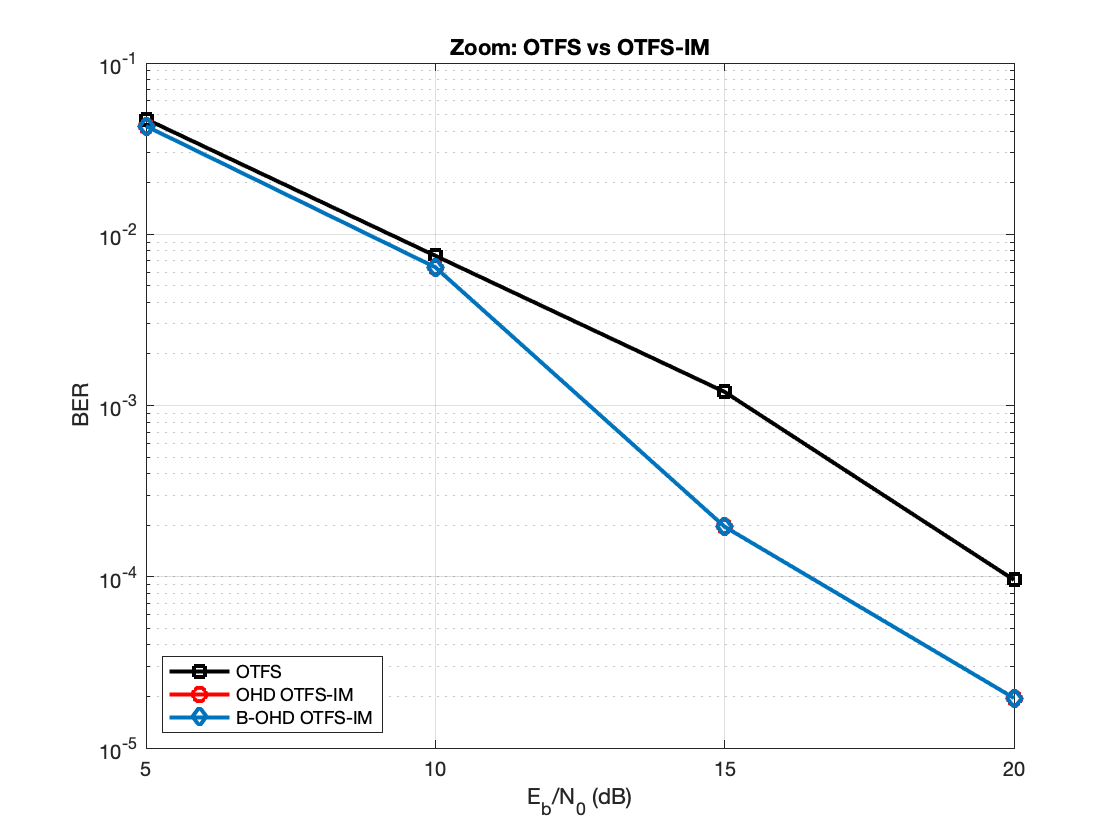
\includegraphics[width=0.88\linewidth]{Images/Chapter5/ber_zoom_n6_k5.png}
    \caption{BER zoom of baseline OTFS and equal-SE OTFS-IM for the \(n=6,k=5\) configuration}
    \label{fig:chapter5_ber_zoom_n6_k5}
\end{figure}
}{%
\begin{figure}[H]
    \centering
    \fbox{\begin{minipage}[c][5cm][c]{0.86\linewidth}
        \centering
        Required figure file is missing:\\
        Images/Chapter5/ber\_zoom\_n6\_k5.png
    \end{minipage}}
    \caption{BER zoom of baseline OTFS and equal-SE OTFS-IM for the \(n=6,k=5\) configuration}
    \label{fig:chapter5_ber_zoom_n6_k5}
\end{figure}
}

Figure~\ref{fig:chapter5_ber_zoom_n6_k5} confirms that the OTFS-IM curves become lower than the baseline OTFS curve from the medium-SNR region onward. At \(5\) dB, the schemes are close because detection is still noise-limited. At \(10\) dB and above, the index-modulated structure begins to provide a measurable BER reduction. Since the spectral efficiency is unchanged, this result is stronger than a lower-rate BER gain.

Another important observation is that OHD and B-OHD overlap in all three equal-SE configurations listed in Table~\ref{tab:chapter5_equal_se_ber_summary}. This does not indicate a plotting error. For \(n=4,k=3\), the number of valid activation patterns is \(\binom{4}{3}=4\), and the number of index-addressable patterns is also four. Therefore, all valid patterns are selected, leaving no additional freedom for B-OHD to improve the table. For \(n=5,k=4\) and \(n=6,k=5\), the valid pattern sets are also highly constrained, so the OHD and B-OHD selection criteria lead to the same effective pattern table.

This result clarifies the role of B-OHD in the thesis. B-OHD is not expected to improve every configuration. Its advantage can only appear when there is enough freedom to choose among multiple candidate pattern sets with the same minimum Hamming distance. In equal-SE configurations with a small or constrained pattern space, OHD and B-OHD may naturally become identical. This is why the \(n=5,k=3\) configuration is later used for pattern-selection validation, while the equal-SE configurations are used mainly to prove that OTFS-IM can improve BER without reducing spectral efficiency.

In summary, the equal-SE results provide the most important evidence for the usefulness of OTFS-IM in this thesis. Across \(4\)-\(3\), \(5\)-\(4\), and \(6\)-\(5\), OTFS-IM maintains the same spectral efficiency as baseline OTFS and still obtains lower BER in the medium and high SNR regions. The improvement is not uniform at all SNR values, but the trend is consistent enough to justify a deeper error-decomposition analysis in the next section.
